\documentclass[border=3mm]{standalone}

\usepackage{tikz}
\usetikzlibrary{arrows.meta}

\begin{document}
	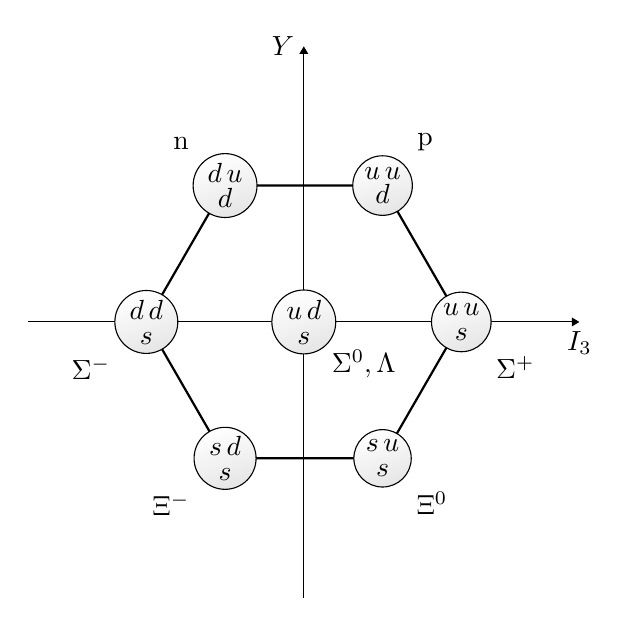
\begin{tikzpicture}[scale=2]
		\tikzstyle{sphere}=[draw,circle,inner sep=1pt,outer sep=2pt,thin,top color=white!50,bottom color=white!90!black,shading angle=20,align=center,minimum size=0.5cm]
		\foreach \i in {0,60,...,300} {
			\coordinate (P\i) at (\i:1); % 1 unit radius from center at angle \i
		}
		\draw[-{Triangle[scale=0.75]}] (-1.75,0) -- (1.75,0) node[below]{$I_3$};
		\draw[-{Triangle[scale=0.75]}] (0,-1.75) -- (0,1.75) node[left]{$Y$};
		\draw[thick] (P0) -- (P60) -- (P120) -- (P180) -- (P240) -- (P300) -- cycle;
		\node[sphere,label={below right,xshift=-3pt,yshift=3pt:$\Sigma^0,\Lambda$}] at (0,0){$u\,d$\\[-3pt]$s$};
		\node[sphere,label={below right:$\Sigma^+$}] at (P0){$u\,u$\\[-3pt]$s$};
		\node[sphere,label={above right:$\mathrm{p}$}] at (P60){$u\,u$\\[-3pt]$d$};
		\node[sphere,label={above left:$\mathrm{n}$}] at (P120){$d\,u$\\[-3pt]$d$};
		\node[sphere,label={below left:$\Sigma^-$}] at (P180){$d\,d$\\[-3pt]$s$};
		\node[sphere,label={below left:$\Xi^-$}] at (P240){$s\,d$\\[-3pt]$s$};
		\node[sphere,label={below right:$\Xi^0$}] at (P300){$s\,u$\\[-3pt]$s$};
	\end{tikzpicture}
\end{document}
